

\section{P-Solution: Max-Cut on Planar Graphs}

\par In 1974, F. Hadlock proved that the maximum cut of a \textit{planar graph} is equivalent to another problem with a known polynomial time algorithm.\cite{Hadlock} A graph is planar if it can be embedded in a plane such that none of its edges cross. Hadlock's result has many practical applications. All forests are planar graphs, as are most geographic maps, many chemical bond charts, and more. I will prove Hadlock's claim, following the same broad steps but using my own arguments.

\begin{figure}[h]
    \centering
    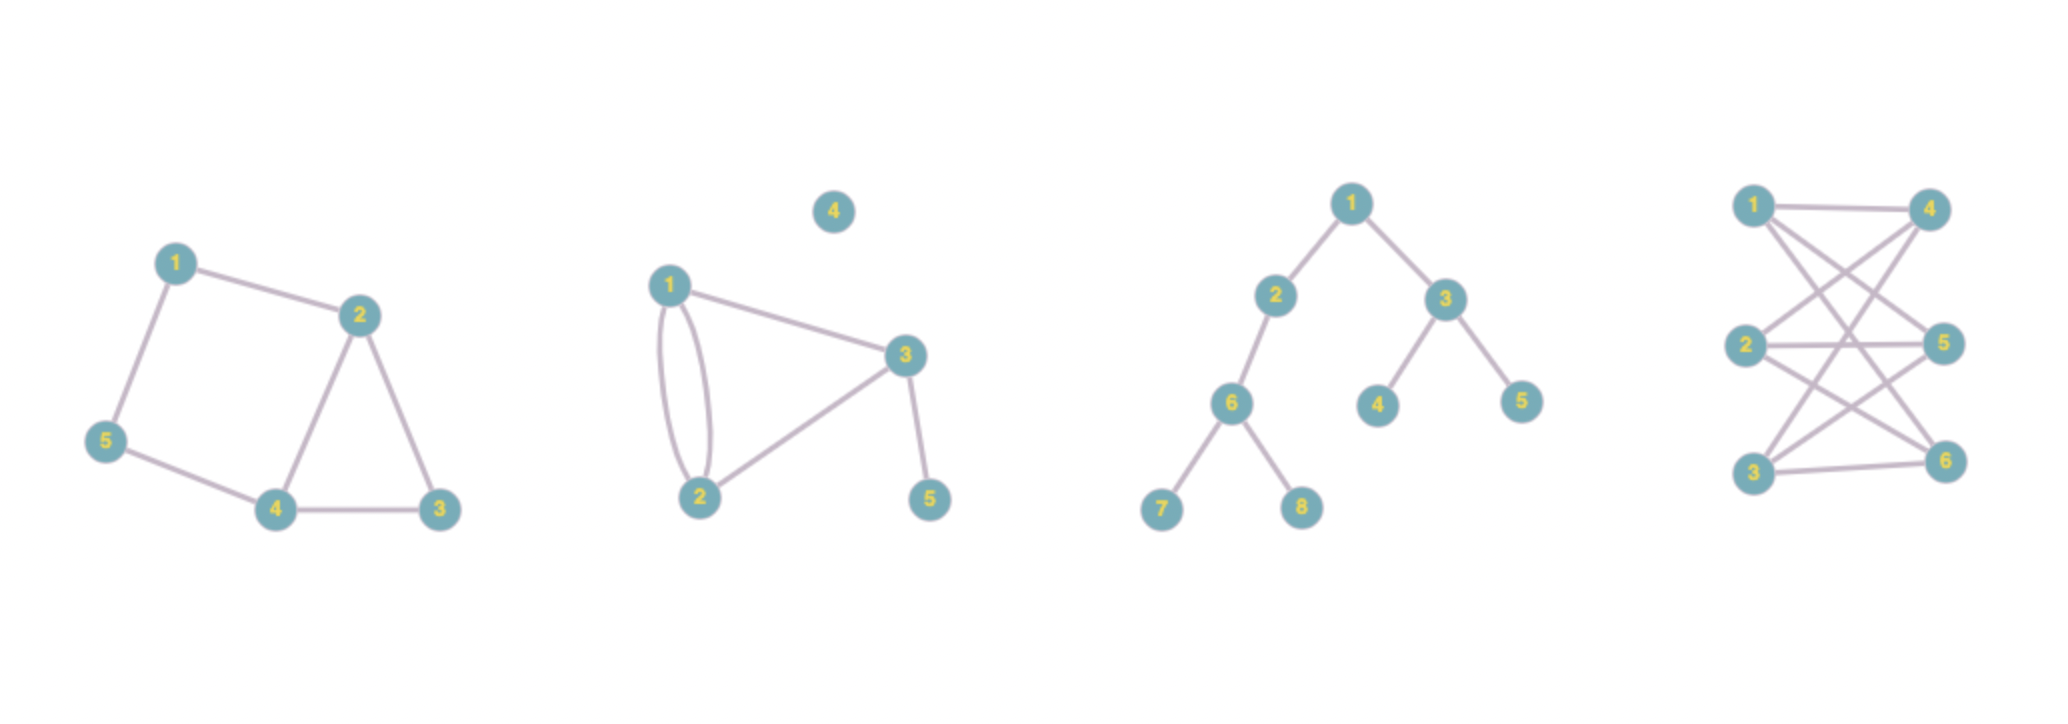
\includegraphics[scale=.35]{planar_examples.png}
    \caption{All of these graphs are planar except the rightmost graph, $K_{3,3}$, whose edges cannot all avoid crossing each other}
    \label{fig:planar_examples}
\end{figure}

\par First, we state some definitions. Given a graph $G$, a \textit{circuit} is a sequence of $m$ distinct edges $\{x_0,x_1\},\{x_1,x_2\},\dots,\{x_{m-1},x_0\}$. The length of a circuit is the number of edges in it. Now consider a subset of the graph's edges $F$. $F$ is an \textit{odd-circuit cover} for $G$ if the graph $G'$ formed by removing $F$ from $G$ has no circuits of odd length. $F$ is an \textit{odd-vertex pairing} if it connects each pair of odd vertices by exactly one path. \\

\begin{lemma}
    The complement of a maximum cut of a graph $G$ is a minimum odd-circuit cover for $G$.\cite{Hadlock}
    \label{lem:max-cut-min-odd-circ}
\end{lemma}

\begin{proof}
    First we will prove that any cut of $G$ is an odd-circuit cover for $G$. Let the set of edges $(S,\bar{S})$ represent a cut of a graph $G$, and let $F_{\alpha}$ be a circuit in $G$. If all vertices in the edges of $F_{\alpha}$ are in the same subset (either $S$ or $\bar{S}$), then $|F_{\alpha} \cap (S,\bar{S})| = 0$, which is even. If we switch one of the vertices to the other side of the cut, its two adjacent edges in $F_{\alpha}$ are either added to or removed from $(S,\bar{S})$, so $|F_{\alpha} \cap (S,\bar{S})|$ will always be even. It follows that any odd circuit in $G$ must have at least one edge outside of the cut. Therefore, the complement of $F_{\alpha}$ is an odd-circuit cover. \\
    
\newpage
    
    For the other direction, consider an arbitrary odd-circuit cover $F_{\beta}$ in $G$. Then its complement $F_{\beta}^{\mathcal{C}}$ contains only even circuits, and therefore only even cycles.\footnote{Cycles are circuits with distinct vertices. Any circuit is made up of one or more cycles, and any cycle is itself a circuit.} By Shahriari's Theorem 10.37,\cite{Shahriari} $E_{OC}^{\mathcal{C}}$ forms a bipartite graph, so all of its edges can be contained in a single cut. \\
    
    We have now proved that any cut of $G$ is an odd-circuit cover for $G$. To prove the original claim, we simply observe that if the sum of weights on a cut is the greatest possible, then the sum of weights on its complement is the least possible.
\end{proof}

\par Here is where planar graphs come in: they have a unique \textit{geometric dual}. Embedding $G$ in a plane partitions it into $k$ faces, and the geometric dual $G_d$ of $G$ has $k$ vertices which each correspond to one of the $k$ faces. For each edge in $G$ that is adjacent to the parts $\alpha$ and $\beta$, the two vertices $v_{\alpha},v_{\beta} \in G_d$ are connected by an edge. The weight of the edge in $G_d$ is the weight of the corresponding edge in $G$.\footnote{Geometric duals can be hard to conceptualize just from reading about them. The example in Section 3.1 should give the reader a more intuitive walkthrough of the process of finding a geometric dual.} \\

\begin{figure}[h]
    \centering
    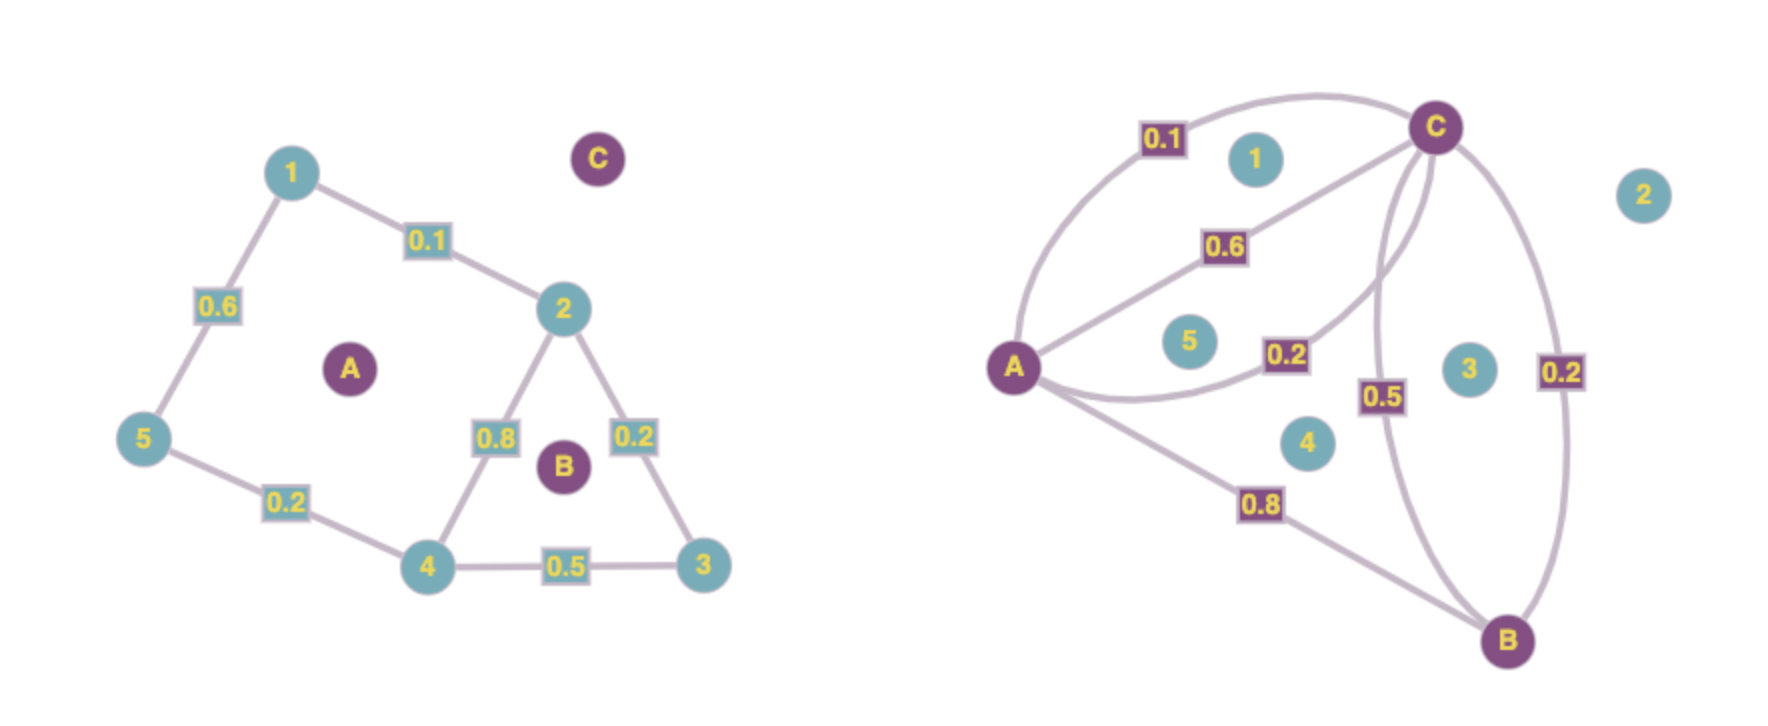
\includegraphics[scale=.35]{geom_dual.png}
    \caption{A planar graph $G$ and its geometric dual $G_d$.}
    \label{fig:geom_dual}
\end{figure}

\par Not only is $G_d$ unique for each embedding of any planar graph $G$, but its geometric dual $(G_d)_d = G$.\cite{hadlock} The reader can visually confirm an example of this in Figure \ref{fig:geom_dual}. Then each subset of edges in $G_d$ is related to exactly one in $G$ that can be found by taking a geometric dual. We take advantage of this fact to find an optimal structure in $G_d$ that corresponds to the minimum odd-circuit cover of Lemma \ref{lem:max-cut-min-odd-circ}.

\newpage

\begin{theorem}
    The maximum cut of a graph $G$ corresponds to the minimum odd-vertex pairing of $G_d$.\cite{Hadlock}
\end{theorem}

\begin{proof}
    Since $\sum_{i=1}^{n} \text{deg}(v_i) = 2|E|$ for any graph, the number of odd-degree vertices in $G$ must be even, so they can be paired off with none left over. An odd-vertex pairing connects each pair of odd-degree vertices by a path. If we remove one of these paths from $G$, the degrees of the two odd-degree vertices on the ends decrease by 1, and the degrees of each vertex in the path decrease by 2. Thus the removal of an odd-vertex pairing leaves a graph with all vertices of even degree. \\
    
    The boundaries of each part of an embedding of $G$ are cycles. Then the vertex $v_i$ of $G_d$ has an edge for each edge in $G$ incident with the $i$th part, so deg$(v_i)$ is the length of the cycle around $i$. Clearly then, if a graph has no odd cycles, its geometric dual has no vertices of odd degree. Therefore, each odd-circuit cover in $G$ corresponds to an odd-vertex pairing in $G_d$, as does each cut in $G$. \\
    
    Furthermore, when the weight of a cut of $G$ is maximized, the weight of the corresponding odd-vertex pairing of $G_d$ is minimized.
\end{proof}

\begin{figure}[h]
    \centering
    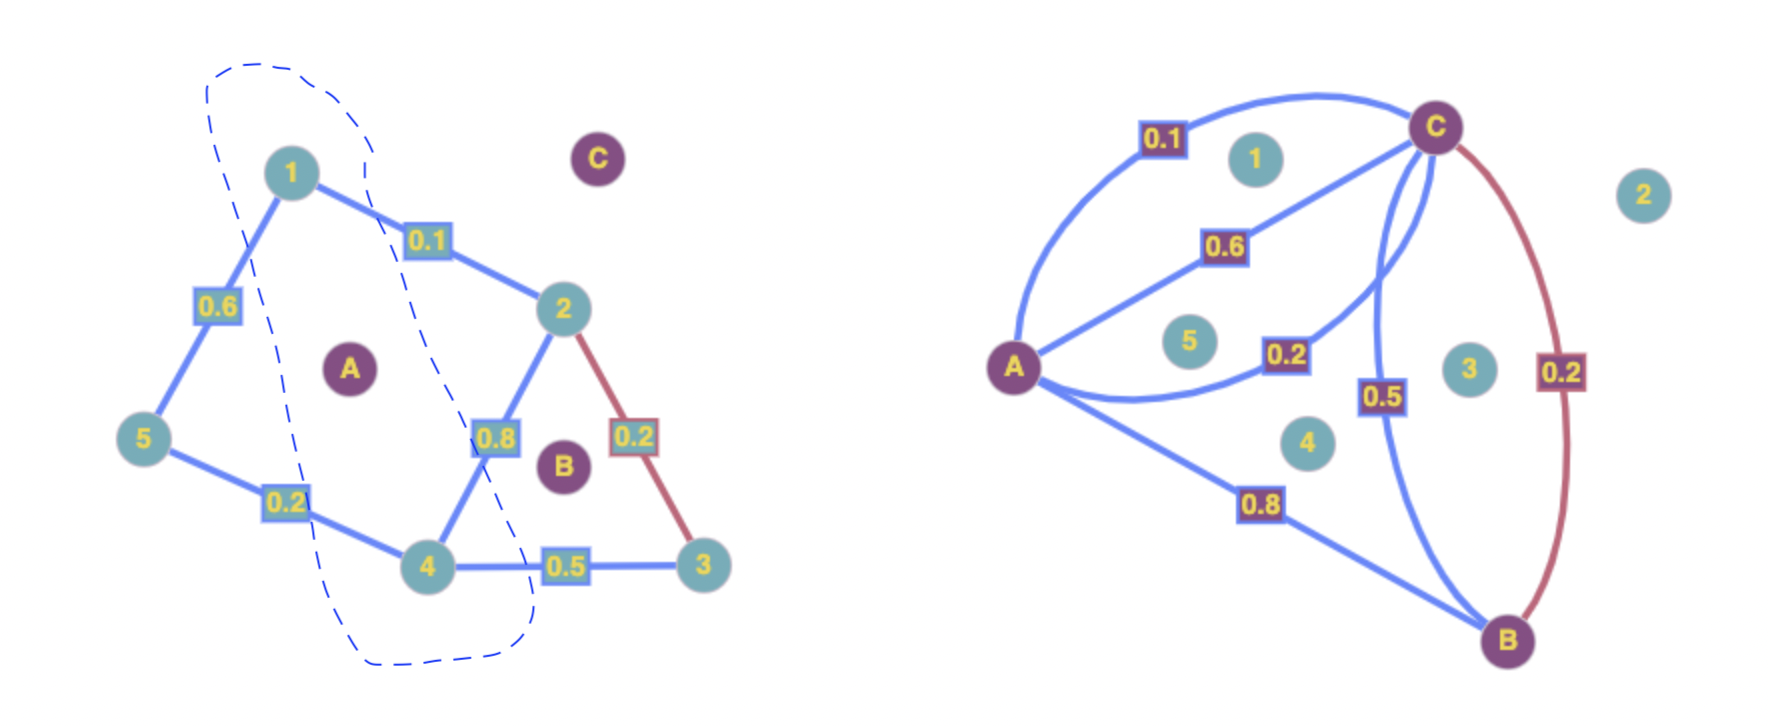
\includegraphics[scale=.35]{geom_dual_cut.png}
    \caption{The minimum odd-circuit cover of $G$ and the minimum odd-vertex pairing of $G_d$ are shown in red, and the maximum cut of $G$ is shown in blue.}
    \label{fig:hadlock_example}
\end{figure}

\par Other researchers have given polynomial-time algorithms for solving the minimum odd-vertex pairing problem.\cite{Hadlock} Since $(G_d)_d = G$ for an embedding of a planar graph $G$, to find the maximum cut of $G$, we need only embed it, run its geometric dual through one of these algorithms, and convert the result by taking the geometric dual once more. Max-cut solutions for non-planar graphs cannot necessarily be found in polynomial time in this manner because they do not necessarily have a unique geometric dual. \\

\newpage

\subsection{Example: Hadlock's Transformation on a Slightly Complicated Planar Graph}

\par For illustration's sake, we will consider the unweighted problem for this example. Consider the graph $G$ and its geometric dual $G_d$ depicted in Figure \ref{fig:slightly_complicated} below.

\begin{figure}[h]
    \centering
    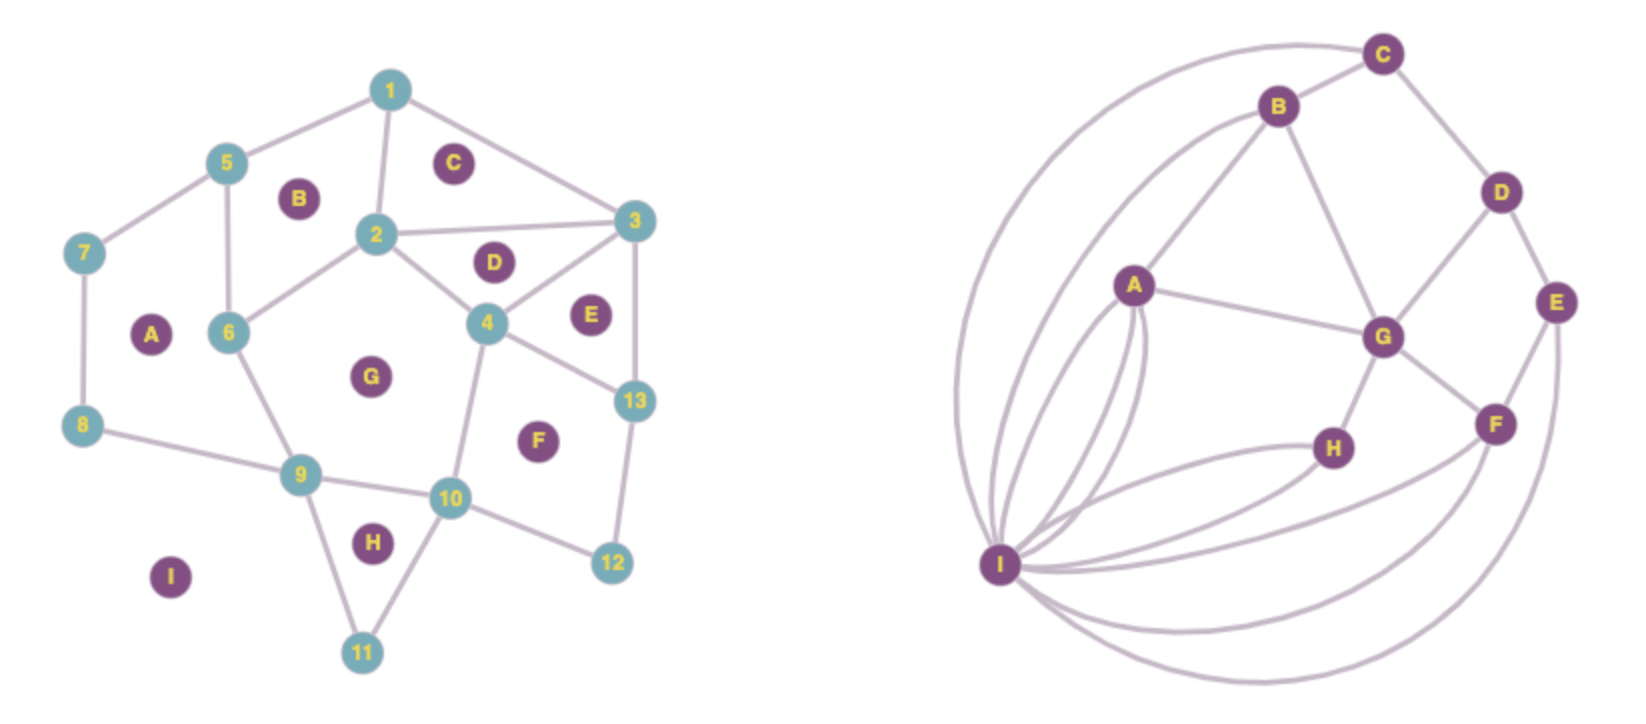
\includegraphics[scale=.35]{planar_dual.png}
    \caption{A planar graph $G$ and its geometric dual $G_d$}
    \label{fig:slightly_complicated}
\end{figure}

\par The vertices of $G_d$ with odd degree are $A$, $C$, $D$, $E$, $G$, and $H$. The reader can confirm visually that the odd-vertex pairing with the fewest edges is $\{(A,B),(B,C),(D,E),(G,H)\}$. This corresponds to the minimum odd-circuit cover in $G$, given by $\{(1,2),(3,4),(5,6),(9,10)\}$. Removing this set of edges indeed eliminates all odd cycles from the graph. And as Figure \ref{fig:slightly_complicated_cut} shows, the complement of this odd-circuit cover is indeed a cut, with a weight of 16. We conclude that this is the maximum cut of $G$.

\begin{figure}[h]
    \centering
    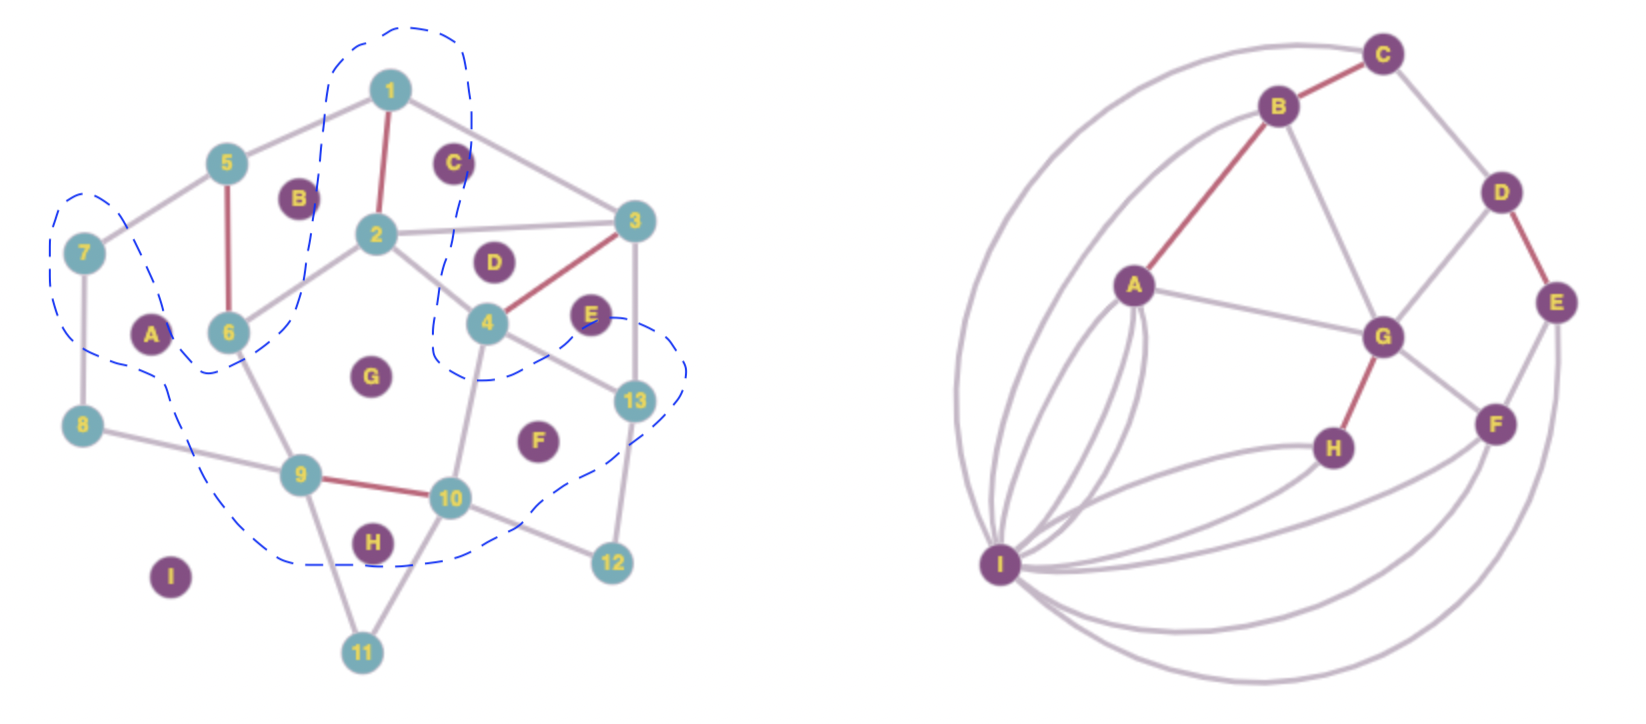
\includegraphics[scale=.35]{planar_dual_cut.png}
    \caption{Using Hadlock's transformation to find the maximum cut of $G$}
    \label{fig:slightly_complicated_cut}
\end{figure}